% -----------------------------------------------------------------
% Document class: Article
\documentclass[ a4paper, twoside, 11pt]{article}
\usepackage{../../../macros-general}
\usepackage{../../../macros-article}
% Number of the handout, quiz, exam, etc.
\newcommand{\numero}{04}
\setcounter{numero}{\numero}

% -----------------------------------------------------------------
\begin{document}
\allowdisplaybreaks

\begin{center}
\Large Mec\'anica Vectorial (MECG-1001): Trabajo Aut\'onomo \numero \\[2ex]
\small \textbf{Semestre:} 2017-2018 T\'ermino II \qquad
\textbf{Instructor:} Luis I. Reyes Castro \qquad
\textbf{Paralelo:} 09
\end{center}
\fullskip

% =============================================
\begin{problem}
\textbf{[4 Puntos]} Los carros de carreras $A$ y $B$ se desplazan sobre porciones circulares de una pista. En el instante que se indica, la rapidez de $A$ disminuye a raz\'on de 7 m/s\tsup{2} y la rapidez de $B$ se incrementa a una tasa de 2 m/s\tsup{2}. Para las posiciones mostradas, determine \textit{(i)} la velocidad de
$B$ relativa a $A$, y \textit{(ii)} la aceleraci\'on de $B$ relativa a $A$.

\begin{figure}[htb]
\centering
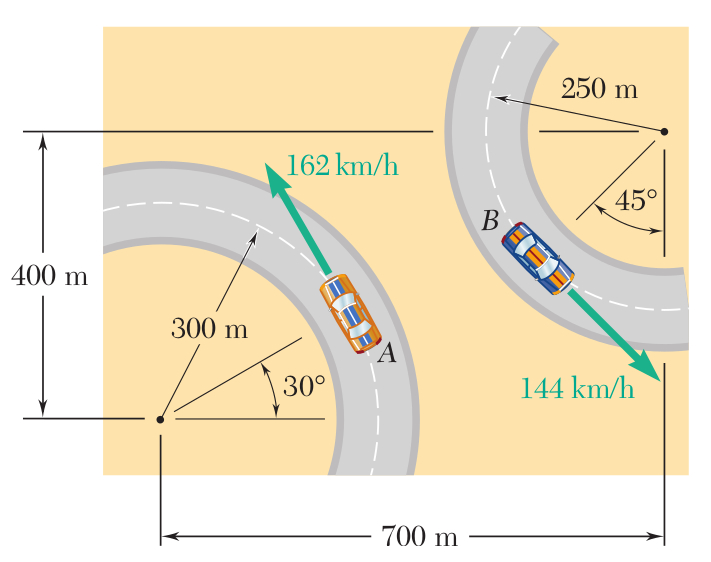
\includegraphics[width=0.5\textwidth]{problema-1.jpg}
\end{figure}

\end{problem}
\fullskip
\fullskip

% =============================================
\begin{problem}
\textbf{[4 Puntos]} La varilla $AB$ se mueve sobre una peque\~na rueda en $C$ mientras el extremo $A$ se desplaza hacia la derecha con una velocidad constante de 500 mm/s. En el instante mostrado, determine \textit{(i)} la velocidad angular de la varilla y \textit{(ii)} la velocidad del extremo $B$ de la varilla.

\begin{figure}[htb]
\centering
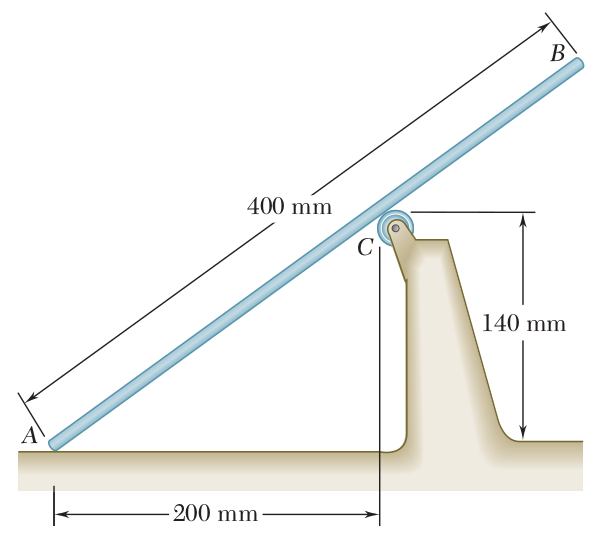
\includegraphics[width=0.5\textwidth]{problema-2.jpg}
\end{figure}

\end{problem}
\fullskip

\end{document}